% Preamble
% ---
\documentclass{article}

% Packages
% ---
\usepackage{amsmath} % Advanced math typesetting
\usepackage[utf8]{inputenc} % Unicode support (Umlauts etc.)
\usepackage[ngerman]{babel} % Change hyphenation rules
\usepackage{hyperref} % Add a link to your document
\usepackage{graphicx} % Add pictures to your document
\usepackage{listings} % Source code formatting and highlighting
\usepackage{booktabs}

\renewcommand{\figurename}{Figure}
%\usepackage[labelsep=endash]{caption}

\usepackage{xcolor}
\lstset { %
    language=C++,
    backgroundcolor=\color{black!5}, % set backgroundcolor
    basicstyle=\footnotesize,% basic font setting
}



\title{%
	MA226 : Monte-Carlo Simulation\\
	 Generation of Multivariate Random Numbers\\
	 \large Assignment 9}

\date{30-03-2017}

\author{%
	Turkhade Hrushikesh Pramod\\
	150123044	}	

\begin{document}

	\maketitle
	\pagenumbering{gobble}
	
	\newpage
	\pagenumbering{arabic}
	
	\section{Problem 1 and 2}
	\paragraph{}
		We have to generate Bivariate Random Numbers for the given parameters.
		
		\paragraph{}
		
			
		
	\subsection{Source code of the solution}
		\lstinputlisting[language=R,firstline=1]{code/que1.R}
		
		\pagebreak
		\subsubsection{Plots}
	
		\paragraph{}
		In the following plots, red line represents Emperical Distribution while blue line represents the actual Distribution.		
		
			\begin{figure}[!ht]
  			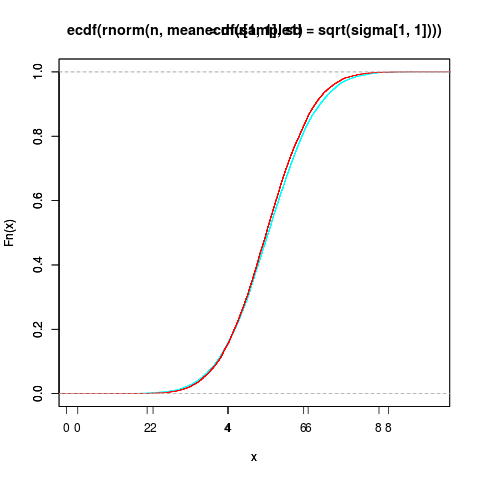
\includegraphics[width=\linewidth]{pic/cdf_sample1_1.png}
 			 \caption{Cumulative Distribution Plot for Sample 1 when a=-0.25}
  			\label{fig:hist1_1}
		\end{figure}
		
		\begin{figure}[!ht]
  			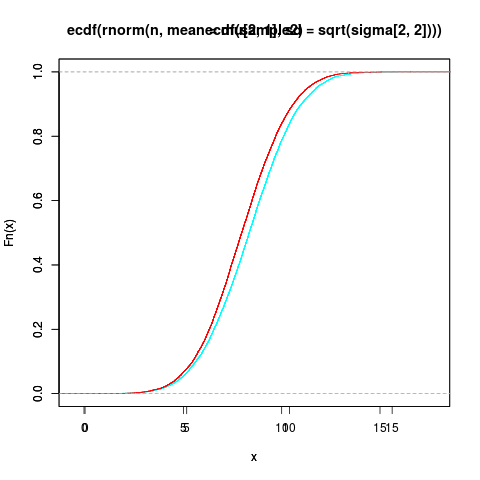
\includegraphics[width=\linewidth]{pic/cdf_sample2_1.png}
 			 \caption{Cumulative Distribution Plot for Sample 2 when a=-0.25}
  			\label{fig:hist1_1}
  			\end{figure}
  			
  			\begin{figure}
  			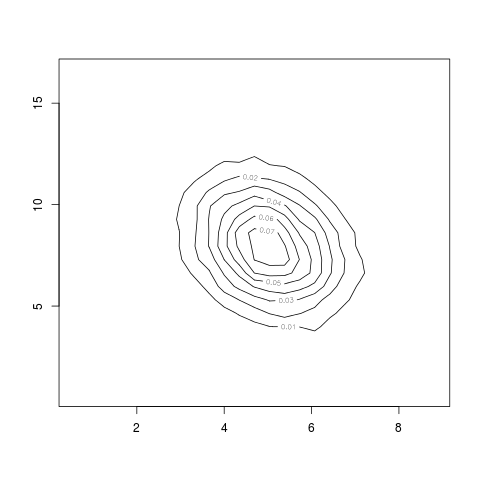
\includegraphics[width=\linewidth]{pic/contour_plot_1.png}
 			 \caption{Contour Plots a=-0.25}
  			\label{fig:hist1_1}
  			\end{figure}
  			
  			\begin{figure}[!ht]
  			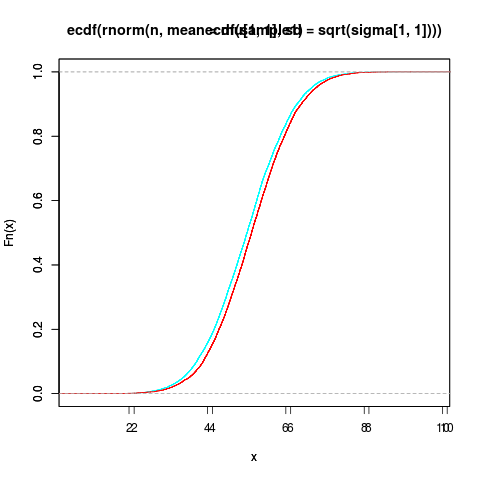
\includegraphics[width=\linewidth]{pic/cdf_sample1_2.png}
 			 \caption{Cumulative Distribution Plot for Sample 1 when a=0}
  			\label{fig:hist1_1}
  			\end{figure}
  			
  			\begin{figure}[!ht]
  			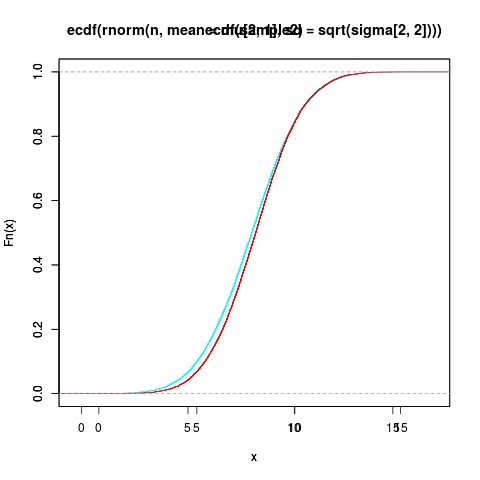
\includegraphics[width=\linewidth]{pic/cdf_sample2_2.png}
 			 \caption{Cumulative Distribution Plot for Sample 2 when a=0}
  			\label{fig:hist1_1}
  			\end{figure}
  			
  			\begin{figure}[!ht]
  			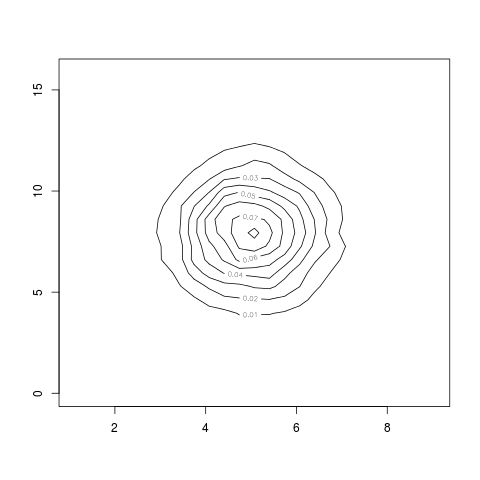
\includegraphics[width=\linewidth]{pic/contour_plot_2.png}
 			 \caption{Contour Plots a=0}
  			\label{fig:hist1_1}
  			\end{figure}
  			
  			\begin{figure}[!ht]
  			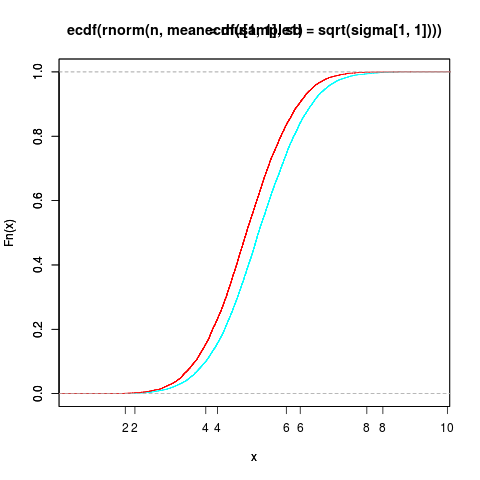
\includegraphics[width=\linewidth]{pic/cdf_sample1_3.png}
 			 \caption{Cumulative Distribution Plot for Sample 1 when a=0.25}
  			\label{fig:hist1_1}
  			\end{figure}
  			
  			\begin{figure}[!ht]
  			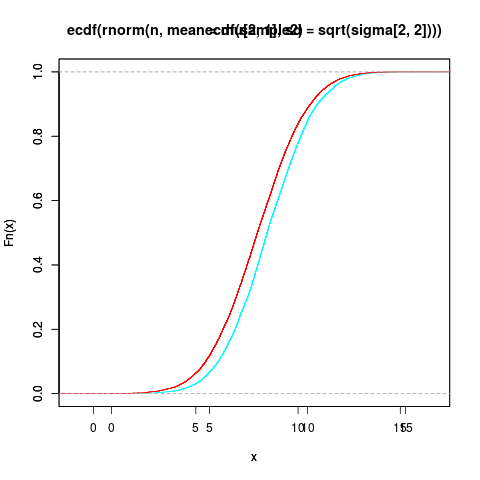
\includegraphics[width=\linewidth]{pic/cdf_sample2_3.png}
 			 \caption{Cumulative Distribution Plot for Sample 2 when a=0.25}
  			\label{fig:hist1_1}
  			\end{figure}
  			
  			\begin{figure}[!ht]
  			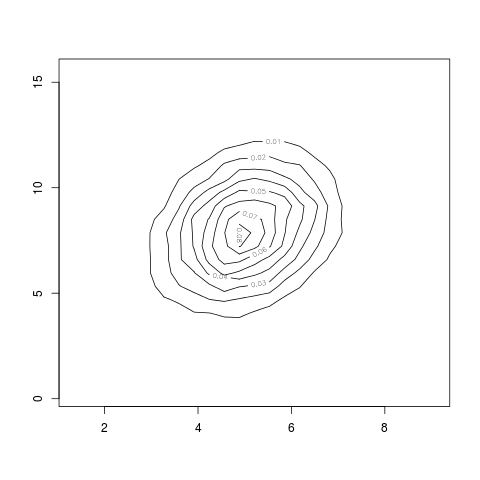
\includegraphics[width=\linewidth]{pic/contour_plot_3.png}
 			 \caption{Contour Plots a=0.25}
  			\label{fig:hist1_1}
  			\end{figure}
		
		\clearpage
		\subsection{Observation}
		\paragraph{}
		
		Calculation for a =  -0.25 \\
Correlation :  -0.2593595 \\

Calculation for a =  0 \\
Correlation :  -0.008781629 \\

Calculation for a =  0.25 \\
Correlation :  0.2582313 \\

	\pagebreak
			
	    \section{Problem 3}
	    \paragraph{}
		We have to generate Bivariate Normal Distribution using Conditioning which has same Parameters as problem before.

			
		
	\subsection{Source code of the solution}			                       \lstinputlisting[language=R,firstline=1]{code/que3.R}
		
		\pagebreak
		\clearpage
		
		\subsection{Observation}
		
Calculatiog for a =  -0.25 \\
Mean vector : [ 5.013493  ,  8.019835 ]\\
Correlation :  -0.2459039 \\

Calculatiog for a =  0 \\
Mean vector : [ 4.99696  ,  7.973594 ]\\
Correlation :  -0.008732466 \\

Calculatiog for a =  0.25 \\
Mean vector : [ 4.999652  ,  8.016126 ]\\
Correlation :  0.2522113\\
		

		

\end{document}